\chapter{Capitolul 6}
\section{Serviciu REST}

Putem defini Representational State Transfer (REST), ca un stil arhitectural situat în partea superioară a unei serii de principii. Creșterea REST în ultimii ani este legată de design-ul API-ului, pe care foarte multe aplicații web îl oferă pentru a extinde funcționalitățile lor. Chiar dacă nu este legat de HTTP, REST este în general asociat cu aplicații web. Se întâmplă ca HTTP să se potrivivească  foarte bine cu principiile REST.
\textbf{Principiile REST sunt:} 
\begin{itemize}
	\item Uniform Interface (interfață uniformă)
	\item  Stateless (fără stare)
	\item Cacheable (se poate salva într-un cache)
	\item Client-Server
	\item  Layered System (sistem stratificat
	\item Code on Demand (cod la cerere)
\end{itemize}

Ideea de REST folosit pe HTTP este de a utiliza funcționalitatea protocolului cât mai mult posibil, astfel încât să nu se reinventeze roata.
\subsection{Uniform Interface}
În „centrul” REST sunt resursele, acele „lucruri” ce se doresc a fi gestionate utilizând API-ul. O resursă poate fi o postare pe blog, un client, un document, și, în general, tot ceea ce se dorește să fie expus. O resursă are un identificator, așa cum o înregistrare în baza de date are o cheie primară. În același fel, o resursă are un URI care identifică resursa.URI-ul nu este o reprezentare a resursei, care poate avea diferite formate, ci este doar un identificator ce poate fi folosit pentru a accesa resursa.
O resursă poate fi solicitată (requested) folosind URI-ul, ceea ce se obține fiind o reprezentare a acestei resurse într-un anumit format. Formatul este negociat între client și server și ar putea fi orice, de la XML și JSON, până la HTML, PNG, CSV sau alte formate binare. Cu reprezentarea resursei, clientul poate manipula starea și poate lucra cu acea resursă, utilizând serverul, dar doar dacă are drepturi să facă acest lucru.
\subsection{Stateless}
Stateless\footnote{fără stare} este un principiu fundamental pentru o aplicație REST; serverul nu ar trebui să stocheze informații despre clienți. Acest lucru înseamnă că, atunci când o cerere ajunge la server, serverul încarcă resursa din spațiul de stocare (de obicei o bază de date) si trimite înapoi reprezentarea resursei către client. Aceasta este starea resurselor. Dacă o secundă mai târziu starea resursei în spațiul de stocare se schimbă datorită unei noi cereri, clientul nu ar trebui să știe de această modificare.
Stateless înseamnă, de asemenea, că serverul nu ar trebui să folosească sesiuni sau alte mecanisme pentru a stoca informații despre client, iar fiecare cerere nu trebuie să fie corelată cu cererile trecute sau viitoare.

\subsection{Cacheable}
Clientul poate „cache-ui” resursa, iar serverul trebuie să ofere informații referitoare la capabilitatea de cache a resursei. Dacă o resursă este „cache-uită” corespunzător, atunci se pot salva câteva ,,round-trip-uri" către server.

\subsection{Client-server}
Singurele lucruri pe care clientul le vede sunt URI-ul și reprezentarea resursei. Clientul nu poate vedea (și cu siguranță nu este interesat în a vedea), unde sunt stocate resursele. Pe de altă parte, serverul nu trebuie să știe dacă clientul are o anumită resursă, iar dacă interfața nu se schimba, cererile între server și client pot fi efectuate fără a fi vreo problemă.
\subsection{Layered System}
Clientul știe foarte puține lucruri despre server; nu știe, de exemplu dacă este direct conectat la server, sau dacă a ajuns la server trecând printr-un proxy sau alt server intermediar (balancer, etc.)
\subsection{Code on Demand}
Serverul poate extinde funcționalitatea clientului prin transmiterea de cod executabil. De exemplu, un server poate trimite JavaScript către client, care poate face un anumit tip de operație asupra datelor.
\paragraph{} Unul din punctele cheie al unui serviciu REST este \textbf{scalabilitatea}. Faptul că serverul nu trebuie să stocheze informații despre client ajută la salvarea memoriei. Sistemul stratificat permite utilizarea de servere cache ca și load-balancer pentru a obține scalabilitate. Adăugarea de noi servere atât timp cât se respectă principiile client-server, permite schimbări de implementare (de exemplu, se poate trece de la o baza de date SQL la una NoSQL) fără știrea clientului.
Dar cum se obține acest lucru și cum funcționează? În majoritatea articolelor, arhitectura REST nu este legată de HTTP, dar HTTP pare perfect pentru a construi un API REST, din moment ce majoritatea lucrurilor pe care REST le definește sunt deja construite chiar în protocol (capabilitatea de a cache-ui, de exemplu).
Web-ul în sine este REST: URL-ul este identificatorul paginii ce se dorește a fi accesată, se introduce URL-ul în browser pentru a obține o reprezentare în format HTML, si se folosește un link pentru a transfera starea la o altă pagină.
\subsection{Operațiile REST}
Un aspect al REST ce este în contrast cu SOAP(RPC) este că o operațiune asupra unei resurse este bazată pe un verb HTTP folosit în combinație cu un URI.
HTTP are noțiunea de verbe. Cele mai folosite sunt GET și POST, dar pe lângă acestea mai sunt câteva ce pot fi utilizate pentru alte operațiuni.
Lista completă a verbelor este: OPTIONS, GET, HEAD, POST, PUT, PATCH, DELETE, TRACE, și CONNECT.
Acestea pot fi folosite cu sensul lor semantic, astfel încât atunci când se citește o resursă, se poate folosi metoda GET, iar atunci când se șterge o resursă, se poate folosi DELETE, și așa mai departe.
\begin{center}
\begin{table}
\begin{tabular}{|c|c|c|}\hiderowcolors
\hline
\cellcolor{LightPink} Operație & \cellcolor{LightGreen} URI & \cellcolor{LightPink} Descriere \\
GET &	\/posts &	Returnează o listă de postări\\
\hline
GET & \/posts/42	& Returnează un singur post(acel post cu id-ul 42)\\
\hline
DELETE & \/posts/42 &	Șterge postul 42.\\
\hline
POST &	\/posts & Adaugă un post.\\
\hline
PUT &	\/posts/42 &	Acutalizează postul 42\\
\hline
PATCH	& \/post/42	& Actualizare parțială \\
\hline
OPTIONS	& \/post/42	& Returnează operațiile ce pot fi efectuate asupra resursei\\
\hline
HEAD &	\/post/42 &	Returnează doar header-ul HTTP\\
\hline
\end{tabular}
\end{table}
\end{center}

După cum se observă în tabelul anterior, folosind URI-ul și verbul corect, o resursă poate fi manipulată folosind operațiile CRUD (Create, Read, Update, Delete).
Atunci când se efectuează o cerere către server, serverul o analizează și construiește răspunsul pentru a returna datele sau rezultatul clientului. Fiecare răspuns este reprezentat de o stare și un status HTTP, ce ar trebui folosit pentru a informa clientul cu privire la rezultatul cererii.
Există cinci tipuri de statuși HTTP:
\begin{itemize}
	\item Informational (1xx)
	\item Succes (2xx)
	\item Redirection (3xx)
	\item Client errors (4xx)
	\item Server errors (5xx)
\end{itemize}

Fiecare tip are propriile detalii. De exemplu, în cazul în care cererea este efectuată cu succes, statusul răspunsului este „200 OK”, după o cerere GET, dar este „201 CREATED” după o cerere POST. În cazul unui client care nu este autorizat să efectueze o cerere, statusul „403 Forbidden” ar trebui utilizat; dacă o resursă nu poate fi găsită, statusul „404 Not found” este utilizat.
\textbf{GET}
GET este folosit pentru a citi o resursă. URI-ul specifică unde se găsește resursa pe care o citim, și se poate folosi header-ul Accept pentru a returna resursa într-un format specific. De exemplu cererea din Figura 1 instruiește serverul să returneze conținutul în format JSON. 
\begin{center}
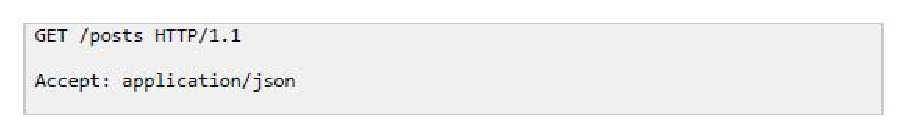
\includegraphics[width=15cm,height=20cm]{imagini/get.eps} 
\caption{Figura1}
\end{center}


Cererea din Figura 2 instruiește serverul să returneze o resursă Post cu identificatorul 42, în format XML.
\begin{center}
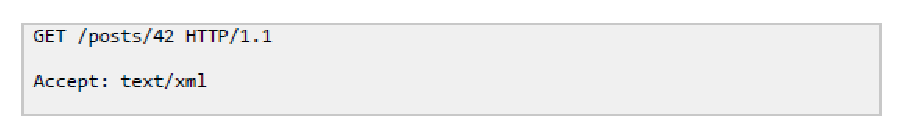
\includegraphics[width=15cm,height=20cm]{imagini/get2.eps} 
\caption{Figura2}
\end{center}

O cerere GET este considerată una sigură, așadar aceasta nu ar trebui să modifice niciodata starea unei resurse.
Serverul răspunde de obicei unei cereri GET cu statusul HTTP 200 OK daca totul decurge bine, 404 Not found dacă URI-ul  pointează către o resură inexistentă, sau 400 Bad request dacă cererea nu este corectă.

\textbf{POST}
Când POST este folosit pentru a crea o resursă, datele resursei sunt trimise către server ca parte a corpului cererii. Serverul răspunde cu un status 201 CREATED dacă totul merge bine. Când este creată o nouă resursă, o bună practică este de a utiliza antetul Location în răspuns pentru a specifica URI-ul resursei nou create. Aceasta bună practică aderă la principiul HATEOAS.

Notă:
HATEOAS (Hypermedia as the Engine of Application State)
Într-o aplicație REST, clientul trebuie să știe cât mai puține informații pentru a utiliza aplicația. În mod ideal, singurul lucru pe care clientul trebuie să îl știe este URI-ul punctuuil de intrare. Toate celelalte URI-uri trebuie să fie furnizate de către server folosind anteturile de localizare sau alte mecanisme (link-uri rel, de exemplu), pentru a informa clientul unde sunt restul resurselor. În acest fel clientul și serverul nu sunt legate și serverul ar putea schimba locația resursei fără a strica clientul. Acest principiu este baza  unui API REST bine conceput.




\textbf{PUT}
PUT este folosit pentru a modifica o resursă. URI-ul specifică resursa care va fi modificată iar corpul cererii conține noile valori ale resursei. Răspunsul ar trebui să conțină statusul 200 OK sau 204 No content în cazul în care răspunsul nu conține resursa modificată. Nu este necesar să se returneze URI-ul resursei în antetul Location deoarece clientul știe deja acest URI. PUT trebuie idempotent, ceea ce înseamnă că rezultatul unei cereri efectuate cu succes nu depinde de numărul de execuții a cererii. Trebuie să fie posibil să se efectueze două apeluri la fel către server, iar serverul nu ar trebui să returneze erori; al doilea apel, pur și simplu actualizează resursa din nou, chiar dacă aceasta nu se schimbă.

\textbf{DELETE}
DELETE este folosit pentru a șterge o resursă. Rezultatul poate fi 200 OK sau 204 NO CONTENT dacă răspunsul nu conține un body. Poate fi 404 Not found dacă URI-ul nu este corect și resursa nu poate fi găsită.


\subsection{ Hello Web API	}

Template-ul  Web API este parte a template-ului de proiect ASP.NET MVC 5. Acesta este instalat implicit in Visual Studio 2012 și Visual Studio 2013. Pentru versiuni mai vechi de Visual Studio aceste template-uri trebuie instalate.
Structura unei aplicații ASP.NET MVC 5 este prezentată în Figura 3.

\begin{center}
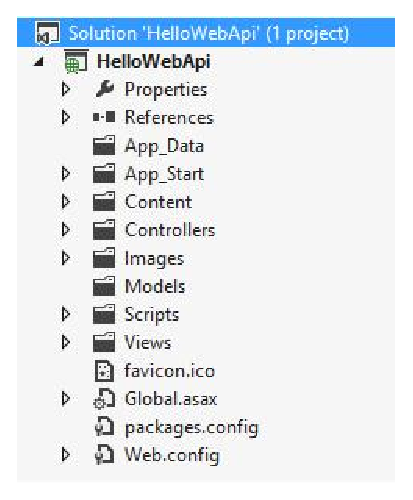
\includegraphics[width=15cm,height=20cm]{imagini/asp.eps} 
\caption{Figura3}
\end{center}

Cele mai importante lucruri de evidențiat sunt:
\begin{itemize}
	\item Directoarele Controllers, Models și Views sunt împrumutate din ASP.NET MVC. Web API folosește același șablon ca și MVC. Totuși, directorul Views nu este foarte folositor în contextul Web API, deși este posibil să se returneze un view către un client.
	\item Pe lângă directorul Views, mai sunt directoarele Images, Scripts și Content. Acestea nu sunt folosite de obicei, din moment ce un API este în general utilizat pentru a returna date, nu interfețe utilizator.
	\item Directorul App Start este folosit pentru a configura API-ul. Acesta conține diverse configurații pentru a seta comportamentul API-ului. 
\end{itemize}
 
Atunci când este creat, un proiect ASP.NET Web API conține un controller implicit. (Figura 4).

\begin{center}
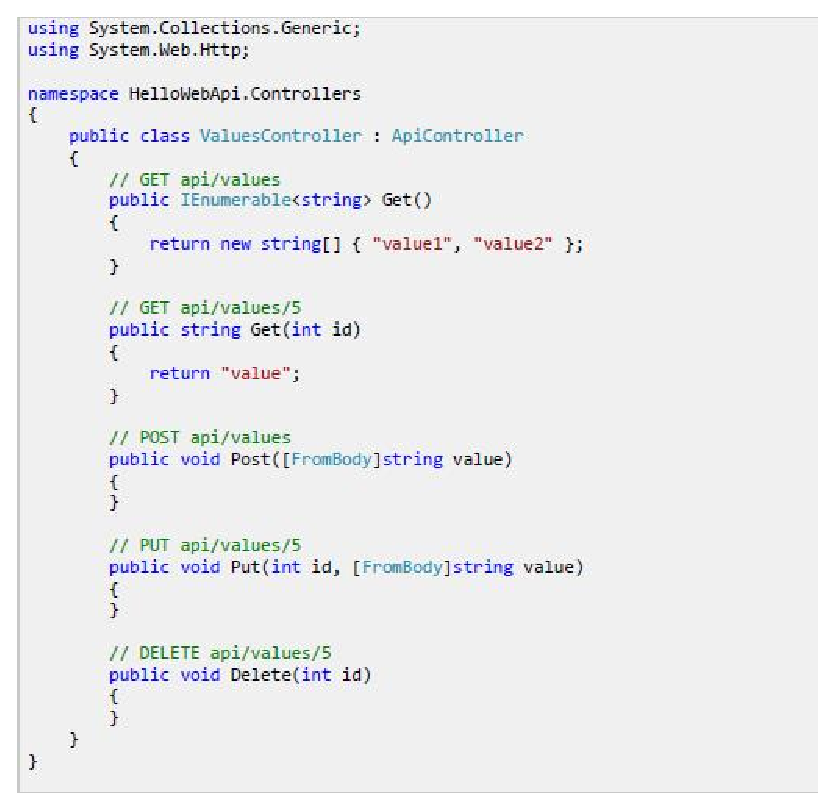
\includegraphics[width=15cm,height=20cm]{imagini/controller.eps} 
\caption{Figura4}
\end{center}
 
După cum se poate vedea în Figura 4, după instrucțiunile "`using"' și "`namespace"' se declară o nouă clasă, ValuesController. Această clasă moștenește din ApiController. Acest lucru este important deoarece, ApiController nu este "`rudă"' cu clasa de bază a controller-or din ASP.NET MVC, chiar dacă au foarte multe similarități. Așadar ApiController deservește ca și clasă de bază pentru toate resursele ce vor fi expuse prin intermediul API-ului.
În interiorul clasei se pot observa toate verbele implicite utilizate în manipularea resurselor: GET, POST, PUT, DELETE. Numele metodelor din interiorul clasei este foarte important, din moment ce runtime-ul ASP.NET Web API folosește convențiile ca pentru a apela metoda corectă, pe care o cerere a formulat-o. Așadar cele două metode Get sunt folosite pentru a returna o colecție de valori și pentru a returna o valoare cu un ID specific. Metodele Post și Put sunt folosite pentru a insera și modifica o resursă, în timp ce metoda Delete este folosită pentru a șterge o resursă cu un id specific.

Ca și o aplicație web ASP.NET MVC, proiectele Web API folosesc un sistem de rutare. Configurarea rutelor se efectuează într-un fișier denumit WebApiConfig.cs, în directorul App Start. Figura 5 ilustrează conținutul acestui fișier.
\begin{center}
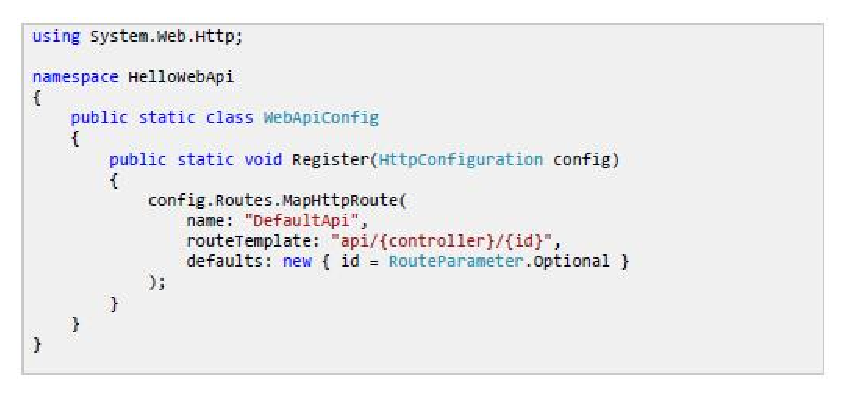
\includegraphics[width=15cm,height=20cm]{imagini/start.eps} 
\caption{Figura5}
\end{center}

Această clasă conține o metodă ce este invocată din clasa WebApiApplication, din global.asax. Această metodă înregistrează rutele folosite de aplicație. Implicit, clasa ValuesController definită în Figura 4, răspunde la URI-ul /api/Values. Este de evidențiat faptul că deși aceste rute sunt similare rutelor din ASP.NET MVC, sunt pe o stivă complet diferită. În cazul Web.API tipul rutei este IhttpRoute iar implementarea este conținută în assembly-ul System.Web.Http, care este un assembly complet nou, ce nu are nicio legătură cu System.Web.
Fiecare rută are un nume și un template ce conține anumiți tokeni pentru a se potrivi cu șabloanele de intrare.

The life of a request

Procesarea unei cereri
Atunci când un client trimite o cerere către o aplicație ASP.NET Web Api, cererea va trece prin trei straturi, pentru a fi procesată. Componentele principale ce au un rol activ în această procesare, sunt listate în Figura 6:
\begin{center}
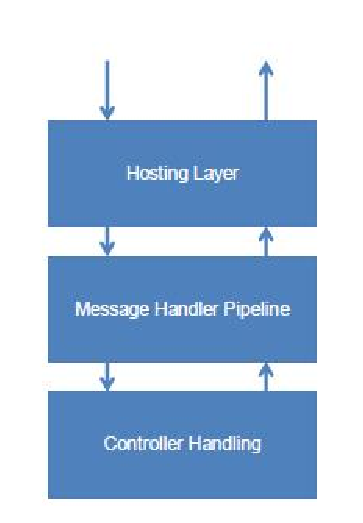
\includegraphics[width=15cm,height=20cm]{imagini/cerere.eps} 
\caption{Figura6}
\end{center}
Următorele straturi sunt folosite atunci când o cerere este procesată:
The Hosting Layer
Primul strat este stratul de hosting, care primește cererea HTTP direct de la client. Stratul de hosting ar putea fi un server clasic de IIS(Internet Information Server) ce folosește mecanismul ASP.NET, sau o aplicație self-hosted.
Rolul stratului de hosting este de a primi cereri și de a le converti în instanțe de HttpRequestMessage, o clasă ce reprezintă cererea. Mesajul cererii este transmis mai jos către Message Handler Pipeline. Cum este contruită această cerere depinde de tipul de hosting.
The Message Handler Pipeline
Message Handler Pipeline reprezintă stratul de mijloc al arhitecturii prezentate. Acesta constă în înlanțuirea  de handlere ce pot fi folosite pentru a satisface nevoile aplicației. Fiecare handler este o instanță a clasei derivată din HttpMessageHandler ce are o metodă, SendAsync, care primește o instanță a HttpRequestMessage și returnează un HttpResponseMessage.
Fiecare din aceste handlere are o referință către un InnerHandler, ce reprezintă următorul handler din secvență ce va fi apelat.
Cu această arhitectură, fiecare cerere poate fi pre-procesată sau post-procesată de multiple handlere ce fac diferite lucruri.
Exemple de handlere de mesaje sunt HttpRoutingDispatcher ce direcționează cererea pe baza unei rute și HttpControllerDispatcher ce trimite cererea către controller.
Aceste handlere sunt deja în secvență, de vreme ce sunt în colecția HttpConfiguration.MessageHandlers. Altele pot fi adăugate în colecție în timpul configurării aplicației Web API.
Controller Handling
Acesta este ultimul strat. Stratul de controller handling primește mesajul cererii de la stratul anterior și apelează acțiunea controller-ului trimițând parametrii ceruți. Task-ul este îndeplinit de HttpControllerDispatcher, ultimul handler din secvență. Acesta, cu ajutorul HttpControllerDescriptor, obține o instanță a clasei ce implementează IHttpInterface și apelează metoda ExecuteAsync a acestei instanțe. Selectarea acțiunii corecte pentru a fi executată intră în îndatoririle metodei ApiController.ExecuteAsync, care bind-uiește parametrii, execută filtrele acțiunii (dacă sunt prezente), iar mai apoi execută acțiunea propriu-zisă.
Un IActionResultConverter convertește rezultatul acțiunii la o instanță HttpResponseMessage. Mesajul cererii este trimis către client folosind aceiași cale ca și cererea.
 


 

